%!TEX root = draft.tex
\section{Parallel algorithms}\label{sec:parallel algorithms}

To achieve a good parallel performance of our numerical solver, we must ensure
the sufficient scalability of all components.  This observation prompted the
dedicated development and optimization of several techniques, which we discuss
in the present section.

\subsection{Grid management}

Adaptive tree-based grids can significantly reduce the computational cost of
level-set methods by restricting the fine grid close to the interface where it
is most needed \cite{Strain:99:Tree-Methods-for-Mov}.
Moreover, adaptive tree-based grids are easy to generate in the presence of a
signed-distance level-set function \cite{Min;Gibou:07:A-second-order-accur} and
can efficiently be encoded using a tree data structure
\cite{Samet:90:Applications-of-Spat}.
In order to develop scalable parallel algorithms on these grids, it is
necessary to parallelize the data structure and grid manipulation methods such
as refinement and coarsening of cells as well as to provide a fast method for
grid partitioning and load balancing.
The \texttt{p4est} library \cite{p4est-github} is a collection of such parallel
algorithms that has recently emerged and shown to scale up to 458,752 cores
%\cite{Burstedde;Wilcox;Ghattas:11:p4est:-Scalable-Algo}.
\cite{IsaacBursteddeWilcoxEtAl15}.

In \texttt{p4est} the adaptive grid is represented as a non-overlapping collection of trees that are rooted in individual cells of a common coarse grid (cf.\ Figure \ref{fig:p4est_zcurve}). This common coarse grid, which we will refer to as the ``macromesh'', can in general be an unstructured quadrilateral mesh, in two spatial dimensions, or hexahedral mesh, in three spatial dimensions.
In this article, however, it is sufficient to limit discussions to simple
uniform Cartesian macromeshes.
Moreover, it is implicitly assumed that the macromesh is small enough that it
can be entirely replicated on all processes.
For instance, in many of the applications that we are considering in this paper the macromesh is simply a single cell.
\texttt{p4est} allows for arbitrary refinement and coarsening criteria through defining callback functions.
In this article the refinement criteria is chosen based on the distance of individual cells to the interface.
Specifically, a cell $C$ is marked for refinement if
\be
\min_{v \in V(C)} |\phi (v)| \le \frac{L D}{2},
\label{eq:refine}
\ee
where $V(C)$ denotes the set of all vertices of cell $C$, $L$ denotes the
Lipschitz constant of the level-set function, and $D$ denotes the diagonal size
of cell $C$.
Conversely, an existing cell is marked for coarsening if
\be
\min_{v \in V(C)} |\phi (v)| > L D.
\label{eq:coarsen}
\ee
We refer to section 3.2 of
\cite{Burstedde;Wilcox;Ghattas:11:p4est:-Scalable-Algo} for details on the
parallel refinement and coarsening algorithms implemented in \texttt{p4est}.

Once the grid is adapted to the interface, it must be partitioned to ensure
load balancing across processes.
This is achieved by constructing a Z-curve that traverses the leaves of all
trees in order of the tree index (cf.\ Figure \ref{fig:p4est_zcurve}).
A Z-curve is a Space Filling Curve (SFC) with the important property that cells
with close Z-indices are also geometrically close (on average) in the physical
domain.
This is beneficial since it leads to both a reduction in MPI communications and
improvements of the cache performance of several algorithms such as
interpolation and finite difference calculations.
For more details on parallel partitioning in \texttt{p4est} one may refer to
section 3.3 of \cite{Burstedde;Wilcox;Ghattas:11:p4est:-Scalable-Algo}.
\begin{figure}[hbtp]
\begin{center}
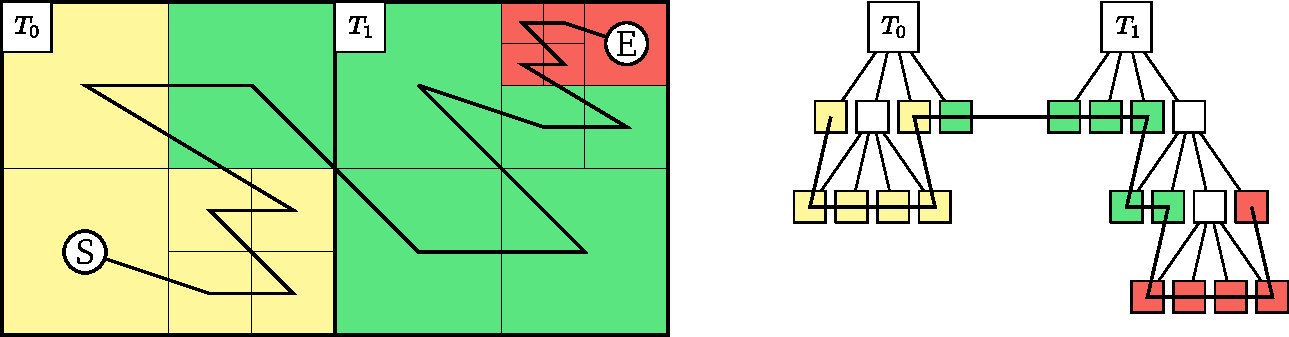
\includegraphics[width = \columnwidth]{figures/p4est_zcurve.pdf}
\caption{Left: a ``forest'' made up of two trees $T_0$ and $T_1$. Parallel
partitioning is achieved by first constructing a Z-curve starting at cell ``S''
and ending at cell ``E''.  Next, the one dimensional curve is split up among
processes either uniformly or by assigning different weights to cells.  Here
processes are represented via different colors.  Note how using the Z-curve
naturally leads to clustering of most cells in each domain.  Right: schematic of
a tree data structure representing this forest and its partitioning.}
\label{fig:p4est_zcurve}
\end{center}
\end{figure}
Aside from grid manipulation and partitioning, we use two additional features
of \texttt{p4est}, namely the generation of ghost layer cells and the creation
of a globally unique node indexing.
These algorithms are detailed in sections 3.5 and 3.6 of
\cite{Burstedde;Wilcox;Ghattas:11:p4est:-Scalable-Algo}.
We have specifically extended the latter algorithm such that it can be applied
to a non-graded refinement pattern.
This is important because we can entirely skip the 2:1 balance function, which
was shown to be one of the most time consuming parts of grid adaptation
in \texttt{p4est}
\cite{Burstedde;Wilcox;Ghattas:11:p4est:-Scalable-Algo}.
% (it has since been optimized \cite{IsaacBursteddeGhattas12}).

Finally, in \texttt{p4est} trees are linearized, i.e.\ only the leaves are explicitly stored. However, explicit knowledge of the hierarchal structure of the tree is greatly beneficial in several algorithms, e.g. in search operations needed for the interpolation algorithm. Thus, we introduce a simple reconstruction algorithm that recreates a local representation of the entire ``forest'' that is only adapted to local cells and, potentially, the ghost layer. This approach is similar to the ideas introduced in \cite{Bangerth;Burstedde;Heister;etal:11:Algorithms-and-data-} and our tests show that in a typical application they amount to less that $1\%$ of the entire runtime. Algorithm \ref{alg:reconstruction} illustrates how this reconstruction is performed. Given a forest and a layer of ghost cells from \texttt{p4est}, the algorithm generates a local representation of the forest by recursively refining from the root until reaching the same level and location of all leaves in the local forest and the ghost layer. Note that algorithm \ref{alg:reconstruction} does not involve any communication and is load balanced provided that the initial forest is balanced. Figure \ref{fig:reconstruction} illustrates an example where Algorithm \ref{alg:reconstruction} is applied. Note how each process has independently generated a local representation of the forest that is refined to match the same leaves as in the global forest and ghost layer.
\begin{figure}[htbp]
\begin{center}
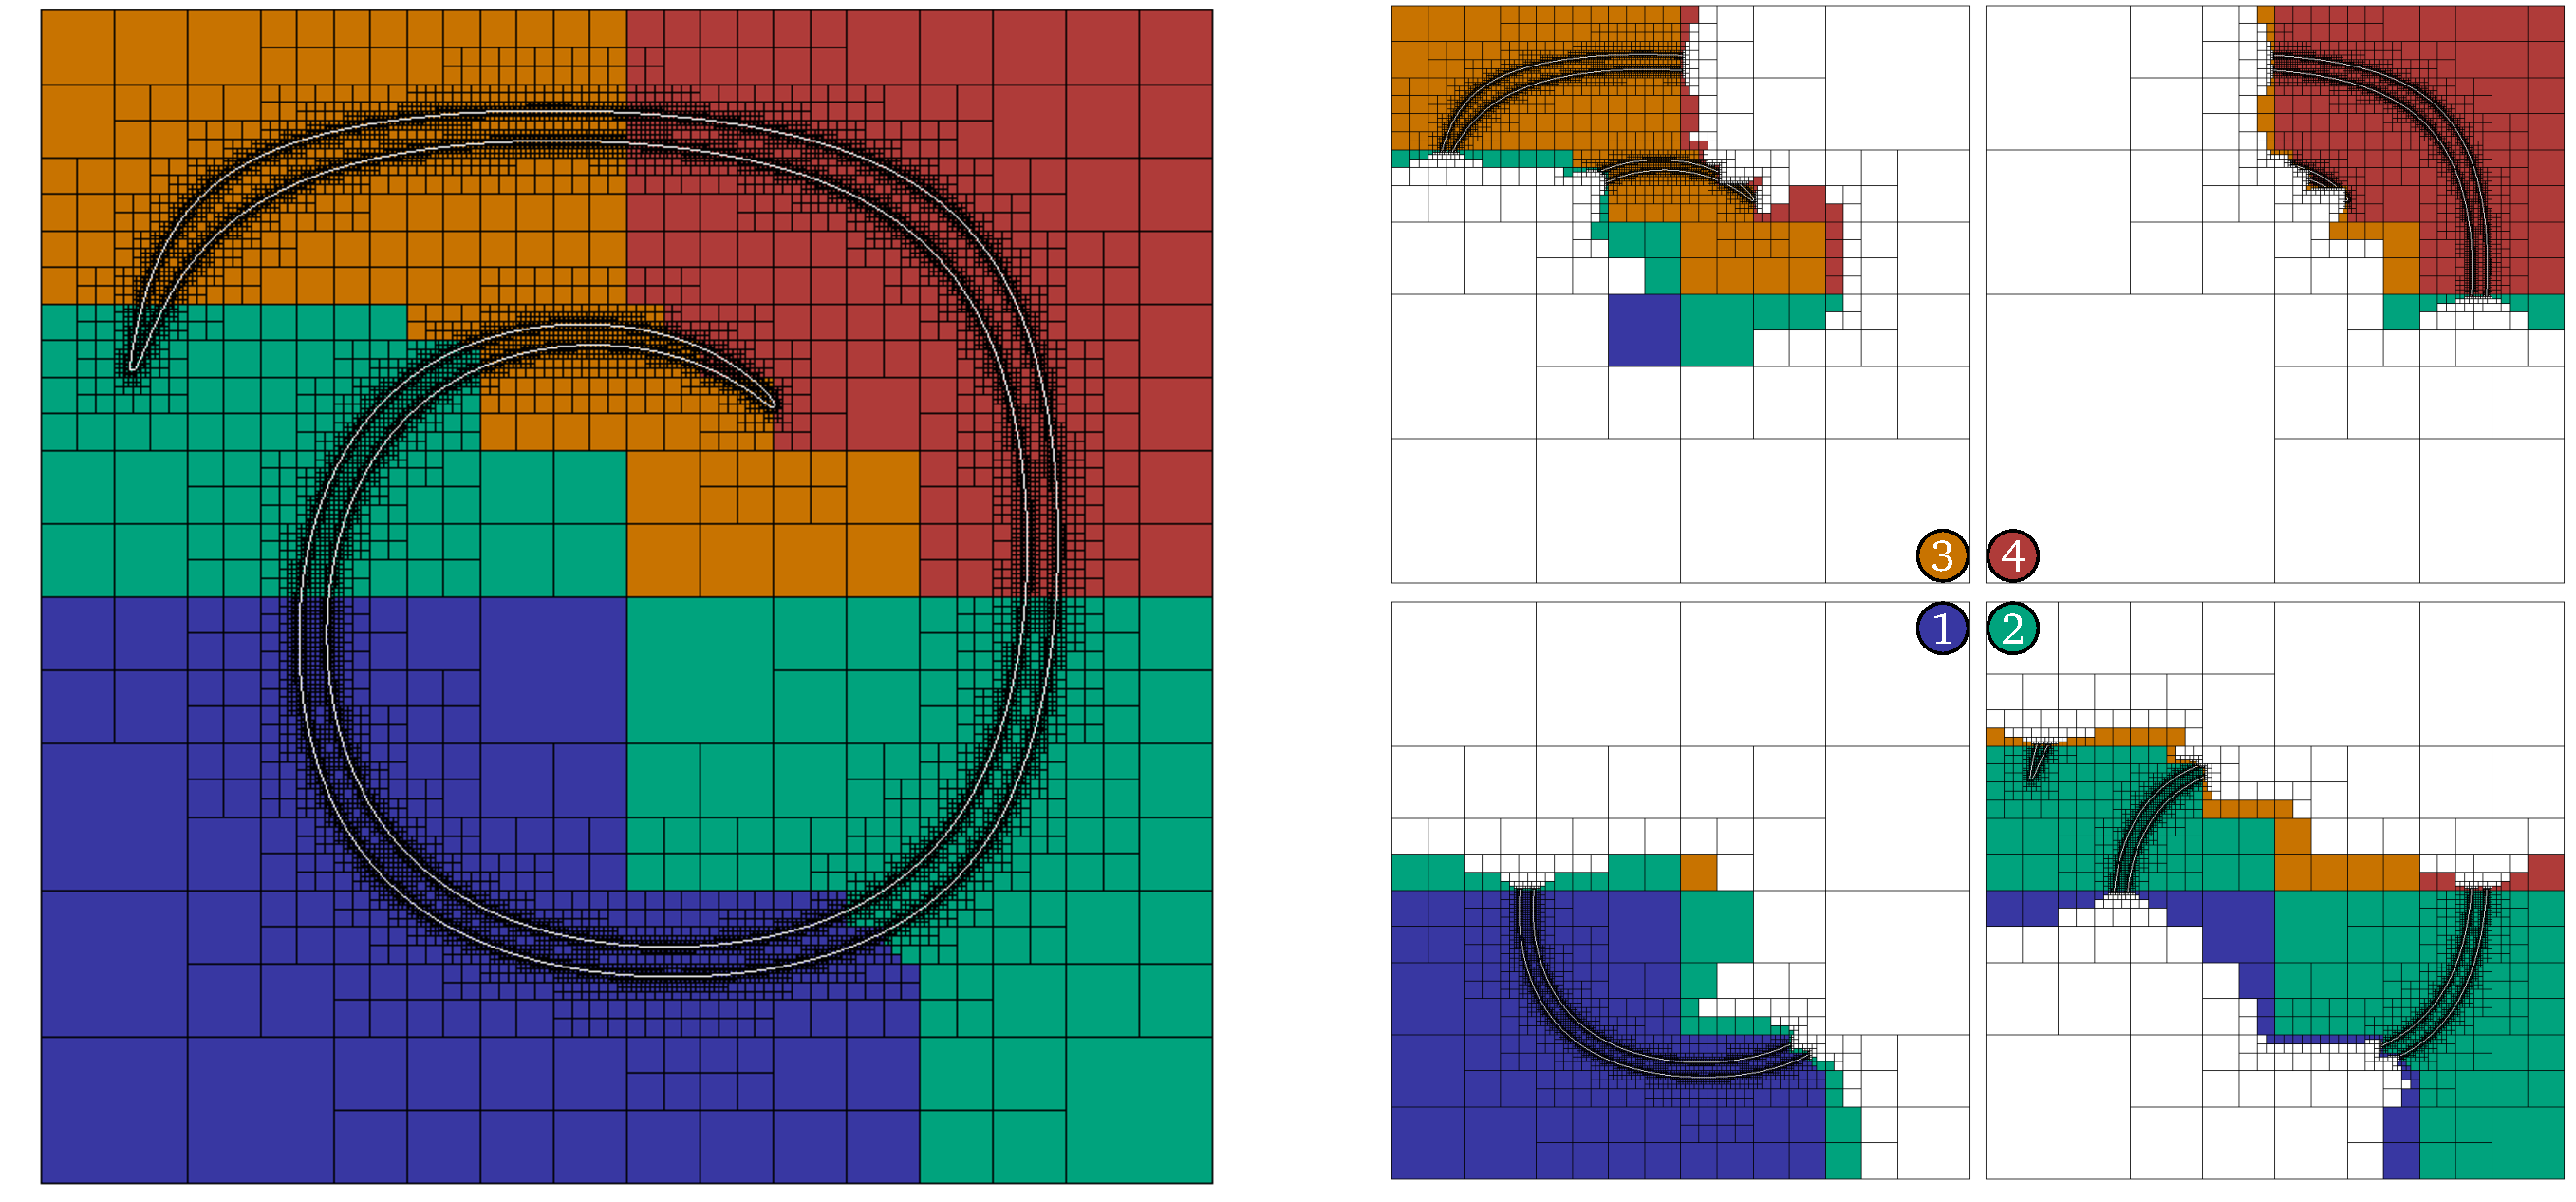
\includegraphics[width = \textwidth]{figures/reconstruct.pdf}
\end{center}
\caption{Left: a forest refined close to an interface and partitioned among four processes, as indicated by colors. Right: each process independently recreates a local forest that is refined to match the local grid and is as coarse as possible elsewhere. Note that empty cells are fictitious, i.e.\ they are only required to generate the hierarchal structure and are not matched by any corresponding cell in the global forest.}
\label{fig:reconstruction}
\end{figure}
\begin{algorithm}[htbp]
\caption{$H \gets \texttt{Reconstruct (}G\texttt{)}$: construction of the local tree hierarchy $H$ from the grid $G$}
\begin{algorithmic}[1]
\State $H \gets G.\texttt{macromesh()}$
\For {$\mathit{tr} : G.\texttt{local\_trees()}$} \Comment{build hierarchy for local cells}
	\For {$c : \mathit{tr}.\texttt{cells()}$}
		\State $H.\texttt{update\_tree(} \mathit{tr}, c \texttt{)}$
	\EndFor
\EndFor

\For {$c : G.\texttt{ghost\_cells()}$} \Comment{build hierarchy for ghost cells}
	\State $H.\texttt{update\_tree(} c.\texttt{tree()}, c \texttt{)}$
\EndFor

\State \Return $H$
\\
\Function{$H.\texttt{update\_tree}$}{$\mathit{tr}, c$}   \Comment{recursive tree reconstruction}
	\State $c_l \gets H.\texttt{root(}\mathit{tr}\texttt{)}$
	\While{$c_l.\texttt{level()} \not= c.\texttt{level()} $}
		\If {$c_l.$\texttt{is\_leaf()}} $c_l$\texttt{.split()}
		\EndIf
		\State $h \gets c_l.\texttt{length()} / 2$ \Comment{select the next child based on direction}
		\State $i \gets c.x \ge c_l.x + h$
		\State $j \gets c.y \ge c_l.y + h$
		\State $k \gets c.z \ge c_l.z + h$

		\State $c_l \gets c_l.\texttt{child(} i, j, k \texttt{)}$
	\EndWhile	
\EndFunction
\end{algorithmic}
\label{alg:reconstruction}
\end{algorithm}

\subsection{Interpolation and semi-Lagrangian methods}
As indicated earlier, we use the semi-Lagrangian method to solve equation \eqref{eq:ls} when the velocity field is externally generated, i.e.\ when it does not depend explicitly on the level-set function itself. Let us rewrite equation \eqref{eq:ls} along the characteristic curve $\underline{\mathbf{X}}(t)$ as:
\be
\left\{
\begin{array}{rcl}
\dfrac{\text{d} \underline{\mathbf{X}}}{\text{d} t} &=& \underline{\mbf{u}}, \\ [3ex]
\dfrac{\text{d} \phi(\underline{\mathbf{X}}(t), t)}{\text{d} t} &=& 0.
\end{array}
\right.
\label{eq:sl}
\ee
The semi-Lagrangian method integrates equations \eqref{eq:sl} backward in time,
i.e.\ starting from the grid $G^{n+1}$ (computed in iteratively as explained
later on), we simply write $\phi^{n+1}(\underline{\mathbf{X}}^{n+1}) =
\phi(\underline{\mathbf{X}}(t^{n+1}), t^{n+1}) =
\phi(\underline{\mathbf{X}}(t^n), t^n) = \phi^n(\underline{\mathbf{X}}_d)$.
Here, the characteristic curves are chosen such that $\underline{\mathbf{X}}(t^{n+1})$ are simply the coordinates of grids points of $G^{n+1}$, and $\underline{\mathbf{X}}_d$ are the departure points, which are computed using the second-order midpoint method \cite{Min;Gibou:07:A-second-order-accur}:
\bea
\underline{\mathbf{X}}^\star &=& \underline{\mathbf{X}}^{n+1} - \frac{\Delta t}{2} \underline{\mbf{u}}^{n}(\underline{\mathbf{X}}^n),	   \label{eq:xstar}      \\
\underline{\mathbf{X}}_d     &=& \underline{\mathbf{X}}^{n+1} - \Delta t \underline{\mbf{u}}^{n+\frac{1}{2}}(\underline{\mathbf{X}}^\star), \label{eq:xdeparture}
\eea
where $\underline{\mbf{u}}^{n+\frac{1}{2}}$ is obtained via extrapolation from previous times, i.e.:
\be
\underline{\mbf{u}}^{n+\frac{1}{2}} = \frac{3}{2} \underline{\mbf{u}}^n - \frac{1}{2}\underline{\mbf{u}}^{n-1}. \label{eq:vn_p_half}
\ee
Note that all values at the intermediate point, $\underline{\mathbf{X}}^\star$,
and departure point, $\underline{\mathbf{X}}_d$, must be calculated via
interpolation from the previous grids $G^{n}$ and $G^{n-1}$.
Here, we use the stabilized second-order interpolation for
$\phi(\underline{\mathbf{X}}_d)$ and the multi-linear interpolation for
$\underline{\mbf{u}}^{n+\frac{1}{2}}(\underline{\mathbf{X}}^\star)$
\cite{Min;Gibou:07:A-second-order-accur}.
Although parallelization of the interpolation process on a shared-memory
machine is trivial, the same cannot be said for distributed-memory machines.
In fact, the parallel interpolation given in Algorithm \ref{alg:interpolation}
is probably the most important contribution of this article since this
procedure, which is trivial on uniform grids, is challenging in the case of
trees because it is not straightforward to identify which processes owns the
departure points.
Indeed, complications arise because not all departure points will reside in the
domain owned by the current process. Moreover, due to the irregular shapes of
the partitions, one cannot even ensure they are entirely owned by neighboring
processes.
At best we can only expect that their locations are bounded by a halo of width
$w \le \text{CFL} \: \Delta x_{\min}$ around the local partition, where
$x_{\min}$ is the size of the smallest cell in the forest.
Naturally, if one enforces $\text{CFL} \le 1$, one can ensure that the halo is
bounded by the ghost layer, which significantly simplifies the communication
problem.
This assumption, however, defeats the purpose of using a semi-Lagrangian
approach, whose purpose is to enable large CFL values.

One remedy to this problem, proposed in \cite{Thomas;Cote:95:Massively-parallel-s} for uniform grids, is to increase the size of ghost layer to $\lceil \text{CFL} \rceil$. For large values of the $\text{CFL}$ number, however, this approach can substantially increase the communication volume. Moreover, this simple approach does not work in the process of generating $G^{n+1}$ due to repartitioning. Indeed, $G^{n+1}$ is built iteratively and load balancing is enforced by repartitioning at each sub-iteration. Therefore, after one such sub-iteration, the backtracked points can end up outside of the initial ghost layer. An alternative approach would be to handle local and remote interpolations separately. Our remote interpolation algorithm is composed of three separate phases. In the first phase, which we call buffering, every process searches for all departure points inside the local trees. If the point is owned by a local cell, it is added to a local buffer, otherwise we find the process which owns the point and add the point to a separate buffer belonging to the found rank. Note that searching the point in the local tree is performed recursively using the hierarchal reconstruction (cf.\ algorithm \ref{alg:reconstruction}). Moreover, the owner's rank is found by computing the Z-index of the point and then using a binary search on the Z-curve. This is already implemented in \texttt{p4est} and explained in details in section 2.5 of \cite{Burstedde;Wilcox;Ghattas:11:p4est:-Scalable-Algo}.

Once buffering is done, every process knows exactly how many messages it needs to send and to which processes. This also implicitly defines processes that will later on send a reply message to this process. However, at this point no process knows which processes to expect a message from. We solve this problem using a simple \textit{communication matrix} (see Figure \ref{fig:communication}). Our approach is very similar to the ``Personalized Census ($\mathcal{PCX}$)'' algorithm described in \cite{Hoefler;Siebert;Lumsdaine:10:Scalable-communication}. Another similar approach is the ``Notify'' algorithm introduced in \cite{Isaac;Burstedde;Ghattas:12:Low-cost-parallel-al}. Furthermore, the MPI-3 standard introduces non-blocking collectives and Remote Memory Access (RMA) operations which enable new ways of solving the communication problem. For instance, authors in \cite{Hoefler;Siebert;Lumsdaine:10:Scalable-communication} descried the ``Non-blocking Consensus ($\mathcal{NBX}$)'' and ``Remote Summation ($\mathcal{RSX}$)'' algorithms which make use of such operations and have better theoretical communication complexities. With the exception of $\mathcal{RSX}$ algorithm, which was not tested in this study, all remaining algorithms produced similar timing and scaling. Thus we have decided to describe our algorithm based on the idea of the \textit{communication matrix}.

\begin{figure}[htbp]
\begin{center}
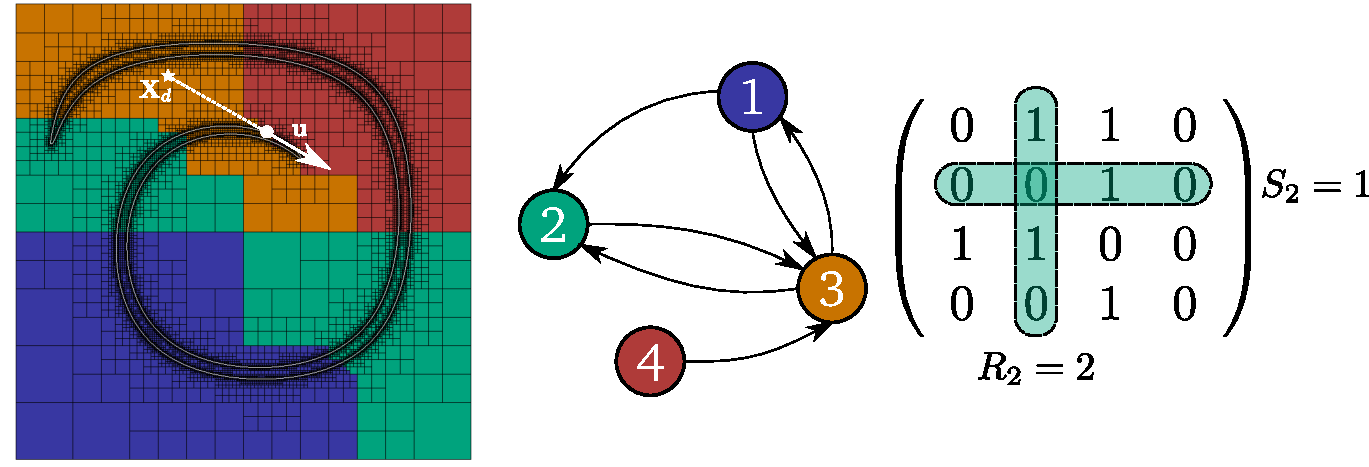
\includegraphics[width = \textwidth] {figures/communication.pdf}
\end{center}
\caption{Left: the location of back-traced points depends on the magnitude of the local velocity and on the time-step. Although the distance to the departure point is bounded by $\text{CFL} \: \Delta x_{\min}$, one cannot predict the receiving rank without explicitly searching the entire Z-curve. Moreover, the receiving process has no prior knowledge about which processes to check for incoming messages nor does it know anything about the possible message length (i.e.\ number of points). Middle: a directed graph illustrating the communication pattern among processes with arrows representing the direction in which messages are sent. Right: the adjacency matrix of the communication graph. For each row, the sum of all columns represents the number of messages that need to be sent. Conversely, for each column, the sum of all rows represents the number of messages that need to be received. As detailed in Algorithm \ref{alg:interpolation}, this information is enough to build a parallel interpolation scheme.}
\label{fig:communication}
\end{figure}

To solve the communication problem, we first compute the adjacency matrix of the communication pattern, i.e.\ we construct the matrix $A_{P \times P}$, where $P$ is the number of processes, such that
\ben
a_{ij} = 
\left\{
\begin{array}{lr}
1 \hspace{5 mm} \text{if process `\textit{i}' sends a message to process `\textit{j}',} \\
0 \hspace{5 mm} \text{otherwise.}
\end{array}
\right.
\een
Note that this matrix is also distributed among processes, i.e.\ each row is owned by a separate rank. Next, we compute
\ben
S_i = \sum_j a_{ij} \hspace{5 mm} \text {and} \hspace{5 mm} R_i = \sum_j a_{ji} ,
\een
where $S_i$ and $R_i$ denote the number of messages sent and received, respectively. While $S_i$ can be computed trivially, a reduction operation is required to compute $R_i$. For instance, this can be achieved using a single \texttt{MPI\_Reduce\_scatter} function call. The last phase of the interpolation procedure involves overlapping the computation of interpolated values for local points with the communication of data between processes. This is done by alternating between local calculations and probing for incoming messages from other processes. The interpolation is finished once the values for all local the points have been calculated and all the remote requests have been processed (see Algorithm \ref{alg:interpolation}).
\begin{algorithm}[htbp]
\caption{$values \gets \texttt{Interpolate (}H, F, \underline{\mathbf{X}}\texttt{)}$: interpolate the value of $F$, defined on the local tree hierarchy $H$, at coordinates $\underline{\mathbf{X}}$}
\begin{algorithmic}[1]
\State $col \gets 0, \mathit{buff} \gets \mathit{null}$ \Comment{Phase I -- buffering}
\For {$\underline{\mathbf{p}} : \underline{\mathbf{X}}$} 
	\State $[r, \mathit{cell})] \gets H.\texttt{search(}\underline{\mathbf{p}}\texttt{)}$ \Comment{search for the owner's rank and cell}
	\If {$r = \mathit{mpirank}$}
        \State $\mathit{buff}[r].\texttt{push\_back(}\underline{\mathbf{p}}, cell\texttt{)}$
	\Else
        \State $\mathit{buff}[r].\texttt{push\_back(}\underline{\mathbf{p}}\texttt{)}$
        \State $\mathit{col}[r] \gets 1$
	\EndIf
\EndFor
\For {$r:\mathit{mpisize}$} \Comment{Phase II -- initiate communication and compute number of messages}
	\If {$\mathit{col}[r]$}
        \State $\texttt{MP\_Isend(}r, \mathit{buff}[r]\texttt{)}$
	\EndIf
\EndFor
\State  $S \gets \texttt{sum(}col\texttt{)}$ 
\State  $R \gets \texttt{MPI\_Reduce\_scatter(}\mathit{col},\texttt{MPI\_SUM)}$
\State $\mathit{done} \gets \mathit{false}, it \gets \mathit{buff}[mpirank].\texttt{begin()}$
\While {$\mathit{!done}$} \Comment{Phase III -- main loop}
	\If {$\mathit{it} \not= \mathit{buff[mpirank]}.\texttt{end()}$}
		\State $\mathit{values} \gets \texttt{process\_local(}it\texttt{)}$ \Comment{process local interpolations}
		\State $\texttt{++}\mathit{it}$
	\EndIf
	\If {$R > 0$} \Comment{process queries sent from remote processes}
		\State $[\mathit{msg, st}] \gets \texttt{MPI\_Iprobe()}$
		\If {$\mathit{msg}$}
			% \State $values \gets \texttt{MPI\_Recv(}st.\texttt{MPI\_SOURCE)}$ \Comment{}
			\State $\mathit{val\_buff} \gets \texttt{process\_queries(}\mathit{st}\texttt{)}$ \Comment{receive, search, and interpolate values}
			\State $\texttt{MPI\_Isend(}\mathit{st}.\texttt{MPI\_SOURCE},\mathit{val\_buff}\texttt{)}$ \Comment{send back interpolated values}
			\State $R\texttt{--}$
		\EndIf
	\EndIf
	\If {$S > 0$} \Comment{process replies sent to our queries}
		\State $\mathit{[msg, st]} \gets \texttt{MPI\_Iprobe()}$
		\If {$\mathit{msg}$}
			\State $\mathit{values} \gets \texttt{process\_replies(}\mathit{st}.\texttt{MPI\_SOURCE)}$ \Comment{receive remotely interpolated values}
			\State $S\texttt{--}$
		\EndIf
	\EndIf
	\State $\mathit{done} \gets S = 0 \: \And \: R = 0 \: \And \: \mathit{it = buff[mpirank]}.\texttt{end()}$
\EndWhile
\State \Return $\mathit{values}$
\end{algorithmic}
\label{alg:interpolation}
\end{algorithm}

Using the interpolation Algorithm \ref{alg:interpolation}, we close this section by presenting the final semi-Lagrangian Algorithm \ref{alg:semi-lagrangian}. The basic idea is to start from an initial guess $G^{n+1}_0$ for the grid and modify it using the refinement \eqref{eq:refine} and coarsening \eqref{eq:coarsen} criteria until convergence is obtained. Various options are available for $G^{n+1}_0$. For instance it is possible to start from the macromesh and only perform refinement steps until convergence. This choice, however, is not suitable since the first few iterations do not contain many cells and there is little work for parallelism. Here we simply take the previous grid as the starting point, i.e.\ $G^{n+1}_0 = G^n$. Note that this iterative process is essentially unavoidable since the grid is based on the values of the level-set function at $t^{n+1}$, which itself is unknown and is to be defined on $G^{n+1}$. Nonetheless the process converges to the final grid in at most $l_{\max}-l_{\min}$ steps where $l_{\min}$ and $l_{\max}$ denote the maximum and minimum depth of all trees in the forest, receptively.
\begin{algorithm}[htbp]
\caption{$[G^{n+1}, \phi^{n+1}] \gets \texttt{SemiLagrangian (}G^n, \phi^n, \underline{\mathbf{u}}^n, \underline{\mathbf{u}}^{n-1}, \text{CFL}\texttt{)}$: update $\phi^{n+1}$ from $\phi^n$ using a semi-Lagrangian scheme and construct the new forest $G^{n+1}$ that is consistent with the zero level-set of $\phi^{n+1}$}
\begin{algorithmic}[1]
\State $\Delta t_l \gets \text{CFL} \times G^n.\texttt{hmin()} / \max \{\underline{\mathbf{u}}^n \} $
\State $\Delta t   \gets \texttt{MPI\_Allreduce(}\Delta t_l,\texttt{MPI\_MIN)}$
\State $H^n \gets \texttt{Reconstruct(} G^n\texttt{)}$ 
\State $G^{n+1}_0 \gets G^n$
\While {$\mathit{true}$}
	\State $\underline{\mathbf{X}}_d  \gets \texttt{ComputeDeparturePoints(}G^{n+1}_0, \underline{\mathbf{u}}^n, \underline{\mathbf{u}}^{n-1}, \Delta t\texttt{)}$ \Comment{using equations \ref{eq:xstar} -- \ref{eq:vn_p_half}}
	\State $\phi^{n+1} \gets \texttt{Interpolate(}H^n, \phi^n, \underline{\textbf{X}}_d\texttt{)}$
	\State $G^{n+1} \gets G^{n+1}_0.\texttt{refine\_and\_coarsen(}\phi^{n+1}\texttt{)}$ \Comment{using equations \ref{eq:refine} and \ref{eq:coarsen} as criteria}
	\If {$G^{n+1} \not= G^{n+1}_0$}
		\State $G^{n+1}.\texttt{partition()}$
		\State $G^{n+1}_0 \gets G^{n+1}$
	\Else
		\State \textbf{break}
	\EndIf
\EndWhile

\State \Return $[G^{n+1}, \phi^{n+1}]$
\end{algorithmic}
\label{alg:semi-lagrangian}
\end{algorithm}

\subsection{Reinitialization}
Successive application of Algorithm \ref{alg:semi-lagrangian}, especially for large values of the CFL number, eventually degrades the signed distance property of the level-set function. Thus, it is important to reinitialize the level-set function every few iterations, especially because the quality of generated grid heavily depends on the signed distance property. To achieve this property we solve the pseudo-time transient equation \eqref{eq:reinitialization} using the discretization scheme detailed in \cite{Min;Gibou:07:A-second-order-accur}. For completeness, we briefly review the scheme. First, we write equation \eqref{eq:reinitialization} in the following semi-discrete form:
\be
\frac{\text{d} \phi}{\text{d} \tau} + S(\phi_0) \left( \mathcal{H}_G(D^+_i \phi, D^-_i \phi) - 1 \right) = 0,
\label{eq:semidiscrete_reinit}
\ee
where $D^+_i \phi$ and $D^-_i \phi$ are the forward and backward derivatives in the $x_i$ direction and $\mathcal{H}_G$ is the Godunov Hamiltonian defined as:
\ben
\mathcal{H}_G(a_i, b_i) = 
\left\{
\begin{array}{lcr}
	\sqrt{\sum_i \max \left(|a^+_i|^2, |b^-_i|^2\right)} & \hspace {5 mm} \text{if} & S(\phi_0) \le 0 ,\\
	\\
	\sqrt{\sum_i \max\left(|a^-_i|^2, |b^+_i|^2\right)} & \hspace {5 mm} \text{if} & S(\phi_0)  >  0 ,
\end{array}
\right.
\een
where $a^+ = \max(a, 0)$ and $a^- = \min(a, 0)$. Similar to \cite{Min;Gibou:07:A-second-order-accur}, equation \eqref{eq:semidiscrete_reinit} is integrated in time using the TVD-RK2 scheme with adaptive time-stepping in order to accelerate the convergence to the steady state. Since the computation is based on a local stencil, the parallel implementation of this scheme is mostly trivial. However, one minor point requires further explanation. As suggested in \cite{Min;Gibou:07:A-second-order-accur}, one-sided derivatives $D^+_i \phi$ and $D^-_i \phi$ are computed using second order discretization which require to compute the second-order derivatives. To enable overlap between computation and communications when computing second-order derivatives and also integrating equation \eqref{eq:semidiscrete_reinit}, we use the following common technique. First, we label all local points, $L_p$, as either private, $P_p$, or boundary, $B_p$. Here, the boundary points are the collection of all local points that are regarded as a ghost point, $G_r$, on at least one other process, i.e.\ $B_p = \underset{r,\;r\neq p}{\bigcup} G_r$. Private points are defined as the collection of all local points that are not a boundary point, i.e.\ $P_p = L_p \setminus B_p$. Algorithm \ref{alg:overlap} illustrates how this labeling can help with overlapping the computation and the communication associated to an arbitrary local operation $y \gets \mathcal{F}(x)$. Note that the \texttt{p4est} library already includes all the primitives required for labeling local points without any further communication.

\begin{algorithm}[htbp]
\caption{$y \gets \texttt{Overlap (}x, \mathcal{F}\texttt{)}$: compute $y_i=\mathcal{F}(x_i)$ for all nodes $i$, where $\mathcal{F}$ is a local operation, while hiding the communication to update the ghost layer}
\begin{algorithmic}[1]
\For {$i:B_p$} \Comment{I -- perform computation on boundary points}
	\State $y_i \gets \mathcal{F}(x_i)$
\EndFor
\State $\mathit{send\_req} \gets \texttt{MPI\_Isend(}y_B\texttt{)}$ \Comment{II -- begin updating ghost values}
\State $\mathit{recv\_req} \gets \texttt{MPI\_Irecv(}y_G\texttt{)}$
\For {$i:P_p$} \Comment{III -- perform computation on private points}
	\State $y_i \gets \mathcal{F}(x_i)$ 
\EndFor
\State $\texttt{MPI\_Waitall(}\mathit{send\_req, recv\_req}\texttt{)}$ \Comment{IV -- wait for ghost update to finish}
\State \Return $y$
\end{algorithmic}
\label{alg:overlap}
\end{algorithm}
